% This file is from Weihao Xia, Jing-Hao Xue. A Survey on 3D-aware Image Synthesis. https://arxiv.org/abs/2210.14267

\documentclass[letterpaper]{article} 
%% tikz作图
\usepackage{tikz}
\usepackage{pgfplots}

\begin{document}
 
\begin{figure*}[th]
\centering
\resizebox{0.90\textwidth}{!}{%
% 这里将第一年yearOne设置为图中起始年,后续就可以直接用年月的形式2019.05直接定义节点的位置
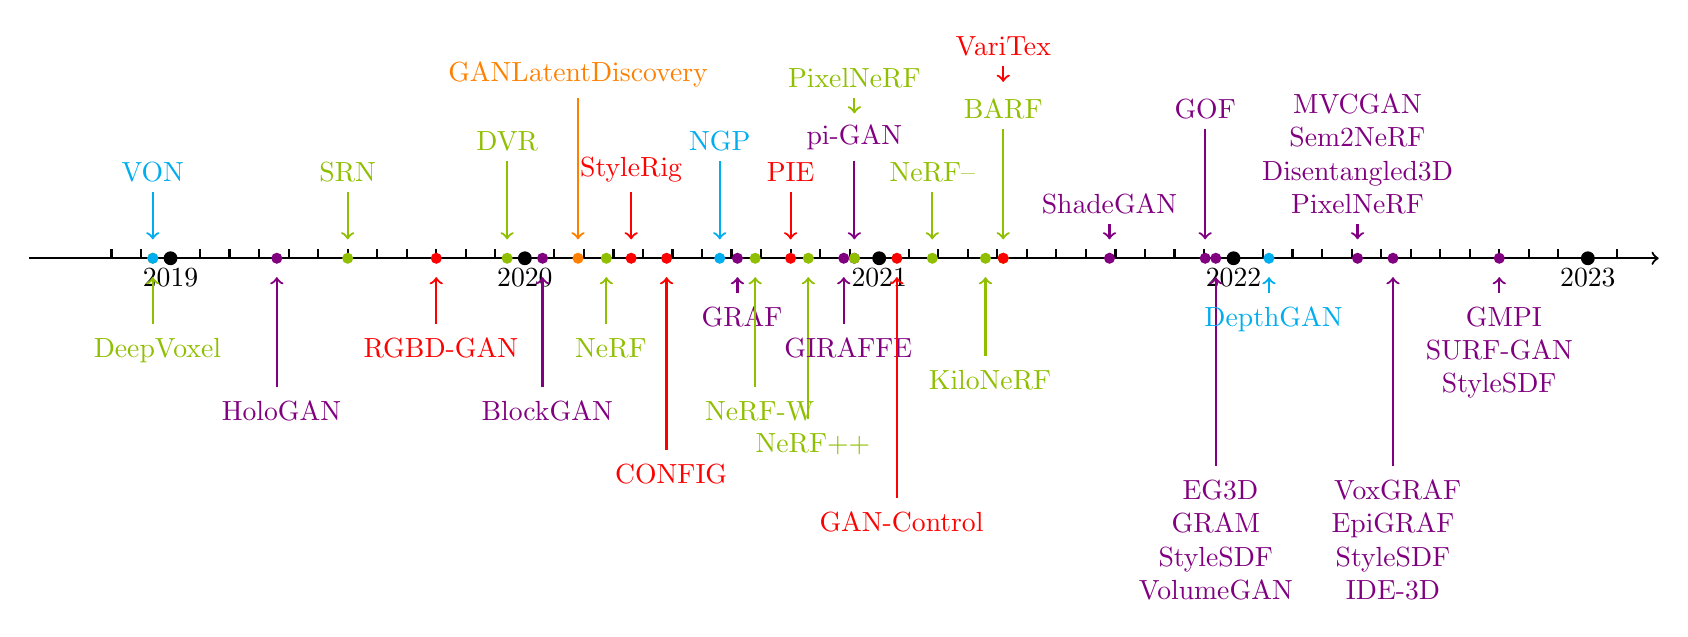
\begin{tikzpicture}%
  \newcount\yearOne; 
  \yearOne= 2019 
  \def\n{4}
  \def\w{18}  
  \def\lt{0.40} 
  \def\lf{0.36} 
  \def\lo{0.12} 
  \def\lext{0.1} 
  \def\rext{1.05} 
  \def\yearLabel(#1,#2,#3){\node[above,black!60!cyan] at ({(#1-\yearOne)*\w/\n},{\lt*#2}) {#3};}

% define yearArrowLabel (#position, #arrow direction(up/down), #arrow length, #method, #color)
    \def\yearArrowLabel(#1,#2,#3,#4,#5){
    \def\xy{{(#1-\yearOne)*\w/\n}}; \pgfmathparse{int(#2*100)};
    \ifnum \pgfmathresult<0 %
      \def\yyp{{(\lt*(0.90+#2))}}; \def\yyw{{(\yyp-\lt*#3)}}
      \fill[color=#5,radius=2pt] (\xy,0) circle;
      \draw[<-,thick,color=#5,align=center]
        (\xy,\yyp) -- (\xy,\yyw)
        node[below,color=#5] at (\xy,\yyw) {\strut #4};
    \else %
      \def\yyp{{(\lt*(0.10+#2)}}; \def\yyw{{(\yyp+\lt*#3)}}
      \fill[color=#5,radius=2pt] (\xy,0) circle;
      \draw[<-,thick,color=#5,align=center]
        (\xy,\yyp) -- (\xy,\yyw)
        node[above] at (\xy,\yyw) {#4};
    \fi}
    
    \draw[->,thick] (-\w*\lext,0) -- (\w*\rext,0);
    
    \foreach \tick in {0,1,...,\n}{
      \def\x{{\tick*\w/\n}}
      \def\year{\the\numexpr \yearOne+\tick*1 \relax}
      \fill[black,radius=2.5pt] (\x,0) circle;
      \draw[thick] (\x,-0.0001) -- (\x,0.0001) %
	               node[below] {\year};
      \ifnum \tick<\n
        \foreach \ticko in {1,2,3,4,5,6,7,8,9,10,11}{
          \def\xo{{(\x+\ticko*\w/\n/12)}}
  	      \draw[thick] (\xo,0) -- (\xo,\lo);  %
	  }\fi
    }
    \draw[thick] (-1*\w/\n/12,0) -- (-1*\w/\n/12,\lo);
    \draw[thick] (-2*\w/\n/12,0) -- (-2*\w/\n/12,\lo);
    \draw[thick] ({\w+\w/\n/12},0) -- ({\w+\w/\n/12},\lo);
  
    \yearArrowLabel(2018.95,-1.5,1.5, DeepVoxel, black!25!lime)  %
    \yearArrowLabel(2018.95,0.5,1.5,VON, cyan)          
    \yearArrowLabel(2019.30,-1.5,3.5, HoloGAN, violet)  %
    \yearArrowLabel(2019.50,0.5,1.5, SRN, black!25!lime) 
    \yearArrowLabel(2019.75,-1.5,1.5, RGBD-GAN, red) 
    \yearArrowLabel(2019.95,0.5,2.5, DVR, black!25!lime) 
    \yearArrowLabel(2020.05,-1.5,3.5, BlockGAN, violet) 
    \yearArrowLabel(2020.15,0.5,4.5, GANLatentDiscovery, orange)
    \yearArrowLabel(2020.23,-1.5,1.5, NeRF, black!25!lime)
    \yearArrowLabel(2020.30,0.5,1.5, StyleRig, red) 
    \yearArrowLabel(2020.40,-1.5,5.5, CONFIG, red) 
    \yearArrowLabel(2020.55, 0.5,2.5, NGP, cyan)   %
    \yearArrowLabel(2020.60,-1.5,0.5, GRAF, violet)  %
    \yearArrowLabel(2020.65,-1.5,3.5, NeRF-W, black!25!lime) 
    \yearArrowLabel(2020.75,0.5,1.5, PIE, red) 
    \yearArrowLabel(2020.80,-1.5,4.5, NeRF++, black!25!lime) 
    \yearArrowLabel(2020.90,-1.5,1.5, GIRAFFE, violet) 
    \yearArrowLabel(2020.93,0.5,2.5, pi-GAN, violet) 
    \yearArrowLabel(2020.93,4.5,0.5, PixelNeRF, black!25!lime) 
    \yearArrowLabel(2021.05,-1.5,7.0, GAN-Control, red)
    \yearArrowLabel(2021.15,0.5,1.5, NeRF--, black!25!lime) 
    \yearArrowLabel(2021.30,-1.5,2.5, KiloNeRF, black!25!lime) 
    \yearArrowLabel(2021.35,0.5,3.5, BARF, black!25!lime) 
    \yearArrowLabel(2021.35,5.5,0.5, VariTex, red) 
    \yearArrowLabel(2021.65,0.5,0.5, ShadeGAN, violet)
    \yearArrowLabel(2021.92, 0.5,3.5, GOF, violet) 
    \yearArrowLabel(2021.95, -1.5, 6.0, EG3D\\GRAM\\StyleSDF\\VolumeGAN, violet) 
    \yearArrowLabel(2022.10, -1.5, 0.5, DepthGAN, cyan) 
    \yearArrowLabel(2022.35, 0.5, 0.5,
    MVCGAN\\Sem2NeRF\\Disentangled3D\\PixelNeRF, violet) 
    \yearArrowLabel(2022.45, -1.5, 6.0, VoxGRAF\\EpiGRAF\\StyleSDF\\IDE-3D, violet) 
    \yearArrowLabel(2022.75, -1.5, 0.5, GMPI\\SURF-GAN\\StyleSDF, violet) 
\end{tikzpicture}
}
\caption{Chronological overview of representative XXX methods which are categorized by different learning approaches. 
Methods in \textcolor{orange}{orange}, \textcolor{red}{red}, \textcolor{cyan}{cyan}, \textcolor{black!25!lime}{lime}, and \textcolor{violet}{violet} are from Section A, B, C, and D, respectively. Best viewed in color.}
\label{fig:timeline} 
\end{figure*}



\end{document}